\documentclass[12pt,a4paper]{article}

% ============================================================
% Encoding and general packages
% ============================================================

\usepackage[utf8]{inputenc}
\usepackage[T1]{fontenc}
\usepackage[brazil]{babel}

\usepackage{fancyhdr}
\usepackage{pdfpages}
\usepackage{mdwlist}
\usepackage{bm}
\usepackage{blindtext}
\usepackage{array}
\usepackage{multicol}
\usepackage{multirow}
\usepackage{enumitem}

% Numerical citations with natbib
\usepackage{natbib}

\usepackage{url}
\usepackage{graphicx}
\usepackage{caption}

\usepackage{amsmath}
\usepackage{amsthm}
\usepackage{amsfonts}
\usepackage{mathrsfs}
\usepackage{amssymb}

\usepackage{mdframed}
\usepackage{xcolor}
\usepackage{fourier-orns}
\usepackage{geometry}
% Proporcoes convencionais de pagina A4, classe nativa article.
% Inclui cabecalho e rodape no calculo das margens para evitar
% o espaco inferior excessivo da configuracao-padrao da classe.
\geometry{
  a4paper,
  left=22.5mm,
  right=22.5mm,
  top=18mm,
  bottom=18mm,
  includeheadfoot
}
\usepackage{parskip}
\usepackage{listings}
\usepackage{setspace}

\usepackage{imakeidx}
\usepackage{etoolbox}

\usepackage{booktabs}
\usepackage{dcolumn}
\usepackage{adjustbox}
\usepackage{subfig}
\usepackage{lscape}
\usepackage{float}
\usepackage{empheq}
\usepackage{tabularx}
\usepackage{longtable}

% Force floats on float-only pages to start at the top
\makeatletter
\setlength{\@fptop}{0pt}
\makeatother

% ============================================================
% Running rules in header and footer
% ============================================================
\setlength{\headheight}{15pt}
\setlength{\headsep}{22pt}
\setlength{\footskip}{36pt}
\fancypagestyle{articlelayout}{%
  \fancyhf{}%
  \fancyhead[L]{\footnotesize\nouppercase{\leftmark}}%
  \fancyhead[R]{\footnotesize Santos-Pereira}%
  \fancyfoot[C]{\thepage}%
  \renewcommand{\headrulewidth}{0.4pt}%
  \renewcommand{\footrulewidth}{0.4pt}%
}
\pagestyle{articlelayout}
\fancypagestyle{plain}{%
  \fancyhf{}%
  \fancyfoot[C]{\thepage}%
  \renewcommand{\headrulewidth}{0.4pt}%
  \renewcommand{\footrulewidth}{0.4pt}%
}
\renewcommand{\sectionmark}[1]{\markboth{\thesection\quad #1}{}}
\fancypagestyle{pprintTitle}{%
  \fancyhf{}%
  \fancyfoot[C]{\thepage}%
  \renewcommand{\headrulewidth}{0.4pt}%
  \renewcommand{\footrulewidth}{0.4pt}%
}


% ============================================================
% Hyperlinks
% ============================================================

\usepackage[
    plainpages=false,
    pdfpagelabels,
    pagebackref=false,
    hyperindex,
    breaklinks=true,
    colorlinks=true,
    citecolor=black,
    linkcolor=black,
    urlcolor=black,
    filecolor=black,
    bookmarksopen=true
]{hyperref}

\pdfstringdefDisableCommands{%
  \def\corref#1{}%
  \def\fnref#1{}%
}
% ============================================================
% Bibliography
% ============================================================

\setcitestyle{numbers,sort&compress}

% ============================================================
% Listings
% ============================================================

\lstset{
    language=Python,
    basicstyle=\fontsize{10}{12}\selectfont\ttfamily,
    keywordstyle=\color{blue},
    commentstyle=\color{green!60!black},
    stringstyle=\color{red},
    showstringspaces=false,
    breaklines=true,
    frame=single,
    numbers=left,
    numberstyle=\tiny\color{gray},
    captionpos=b,
    escapeinside={(*@}{@*)}
}

% ============================================================
% General mathematical definitions
% ============================================================

\DeclareMathOperator{\sech}{sech}

\newcommand{\sen}{\mathrm{sen}}
\newcommand{\dd}{\mathrm{d}}

\newcommand{\keywords}[1]{%
    \textbf{\textit{keywords:}} #1%
}

\newcommand{\palavraschave}[1]{%
    \textbf{\textit{palavras-chave:}} #1%
}

\newcommand{\EE}{\mathbf{e}}
\newcommand{\RR}{\mathrm{R}}
\newcommand{\GG}{\mathbf{G}}
\newcommand{\TT}{\mathrm{T}}

% ============================================================
% Geometry notation for this paper
% ============================================================

% Point
\newcommand{\pt}[1]{\mathbf{#1}}

% Segment
\newcommand{\seg}[1]{\mathbf{#1}}

% Positive segment length
\newcommand{\seglen}[1]{\lvert\mathbf{#1}\rvert}

% Directed segment
\newcommand{\dseg}[1]{\overline{\mathbf{#1}}}

% Power of a point
\DeclareMathOperator{\Pot}{Pot}

% ============================================================
% Equation shortcuts
% ============================================================

\newcommand{\be}{\begin{equation}}
\newcommand{\ee}{\end{equation}}

\newcommand{\beq}{\begin{eqnarray}}
\newcommand{\eeq}{\end{eqnarray}}

\newcommand{\lb}[1]{\label{#1}}

% ============================================================
% Additional personal definitions
% ============================================================

\newcommand{\up}[1]{%
    \raisebox{0.7mm}{$\scriptstyle\,#1$}%
}

\newcommand{\dn}[1]{%
    \raisebox{-0.7mm}{$\scriptstyle #1$}%
}

\newcommand{\upb}[1]{%
    \raisebox{0.5mm}{$\scriptstyle #1$}%
}

\newcommand{\sty}{\scriptstyle}
\newcommand{\ssty}{\scriptscriptstyle}
\newcommand{\tsty}{\textstyle}

\newcommand{\apg}{\:^{>}_{\sim}\:}
\newcommand{\apl}{\:^{<}_{\sim}\:}

\newcommand{\eg}{{\it e.g.\ }}
\newcommand{\ie}{{\it i.e.\ }}

\newcommand{\Px}{\mathcal{P}(x)}
\newcommand{\e}{{\mathrm{e}}}

\newcommand{\dl}{d_{\ssty L}}
\newcommand{\dlzero}{d_{\ssty L_0}}

\newcommand{\Vl}{V_{\ssty L}}

\newcommand{\da}{d_{\ssty A}}
\newcommand{\dg}{d_{\ssty G}}
\newcommand{\dz}{d_z}

\newcommand{\tb}{t_{\ssty B}}
\newcommand{\rb}{r_{\ssty B}}

\newcommand{\gaml}{\gamma_{\ssty L}}
\newcommand{\gama}{\gamma_{\ssty A}}
\newcommand{\gamg}{\gamma_{\ssty G}}
\newcommand{\gamz}{\gamma_{\ssty z}}

\newcommand{\df}{\mathrm{d}}

\newcommand{\obs}[1]{%
    [#1]_{{\tsty{\ssty\rm obs}}}%
}

\newcommand{\dobs}{%
    d_{{\tsty{\ssty\rm obs}}}%
}

\newcommand{\Nobs}{%
    N_{{\tsty{\ssty\rm obs}}}%
}

\newcommand{\Vobs}{%
    V_{{\tsty{\ssty\rm obs}}}%
}

\newcommand{\gobs}{%
    \gamma_{{\tsty{\ssty\rm obs}}}%
}

\newcommand{\bigobs}[1]{%
    \left[#1\right]_{{\tsty{\ssty\rm obs}}}%
}

\newcommand{\Mbar}{\bar{M}}
\newcommand{\etal}{\textit{et al.\ }}

% ============================================================
% Circled-symbol definitions
% ============================================================

\makeatletter

\newcommand{\oz}{%
    \mathbin{\mathpalette\make@circled{z}}%
}

\newcommand{\odl}{%
    \mathbin{\mathpalette\make@circled{\dl}}%
}

\newcommand{\ogams}{%
    \mathbin{\mathpalette\make@circled{\gaml^\ast}}%
}

\newcommand{\make@circled}[2]{%
    \ooalign{%
        $\m@th#1\smallbigcirc{#1}$\cr
        \hidewidth$\m@th#1#2$\hidewidth\cr
    }%
}

\newcommand{\smallbigcirc}[1]{%
    \vcenter{%
        \hbox{%
            \scalebox{1.6}{$\m@th#1\bigcirc$}%
        }%
    }%
}

\makeatother

% ============================================================
% natbib citation separator customization
% ============================================================

\makeatletter
\def\NAT@def@citea{%
    \def\@citea{\NAT@separator}%
}
\makeatother

% ============================================================
% Numbering
% ============================================================

\numberwithin{equation}{section}

% ============================================================
% Theorem environments
% ============================================================

\newtheorem{exercise}{Exercício}[section]
\newtheorem{definition}{Definição}[section]
\newtheorem{example}{Exemplo}[section]

\newtheorem{theorem}{Teorema}[section]
\newtheorem{proposition}{Proposição}[section]
\newtheorem{corollary}{Corolário}[section]

\theoremstyle{remark}
\newtheorem{remark}{Observação}[section]

% ============================================================
% Index
% ============================================================

\makeindex


\begin{document}

\title{Potência de um Ponto e Aceleração Centrípeta:\\
\large Da Geometria Exata da Circunferência à Cinemática Local}
\author{Osvaldo L.\ Santos-Pereira\thanks{\textbf{ORCID:} \href{https://orcid.org/0000-0003-2231-517X}{0000-0003-2231-517X}. \textbf{E-mail:} \href{mailto:olsp@if.ufrj.br}{olsp@if.ufrj.br}.}\\
\small Instituto de Física, Universidade Federal do Rio de Janeiro (UFRJ)\\
\small Rio de Janeiro, Brasil}
\date{}
\maketitle
\begin{abstract}
Este trabalho apresenta uma correspondência entre uma conhecida derivação geométrica da aceleração centrípeta e uma configuração clássica da geometria plana. O problema físico é o movimento circular uniforme, compreendido localmente como o desvio contínuo do movimento tangencial inercial em direção ao centro de curvatura. A identidade relevante entre produtos de segmentos é a relação tangente--secante, já contida na geometria euclidiana clássica; a contribuição de Steiner, em 1826, consistiu em introduzir a noção unificadora de potência de um ponto. O artigo revisa a literatura histórica e pedagógica, emprega as relações geométricas clássicas necessárias à comparação, reúne suas demonstrações usuais no Apêndice A e esclarece o caráter local de sua aplicação à aceleração centrípeta. Em particular, o desvio geométrico auxiliar $h_g$ e o desvio normal físico $h_c$ coincidem até a ordem quadrática no tempo e passam a diferir na quarta ordem. Com $\tau=vt/R$, a discrepância relativa entre eles é $(h_g-h_c)/h_c=-\tau^2/6+O(\tau^4)$, o que fornece uma medida quantitativa da validade da construção em tempos curtos. O tratamento destina-se a estudantes de graduação em mecânica e estabelece uma ponte geométrica entre o movimento circular uniforme, a aceleração instantânea e a geometria euclidiana clássica.
\end{abstract}

\noindent\textbf{Palavras-chave:} aceleração centrípeta; Huygens; Newton; potência de um ponto.

\clearpage
\thispagestyle{plain}

% ============================================================
% Glossary
% ============================================================

\phantomsection
\addcontentsline{toc}{section}{Glossário}

{\LARGE\bfseries Glossário}

\vspace{1.4em}

\begingroup
\footnotesize
\renewcommand{\arraystretch}{1.04}
\setlength{\tabcolsep}{6pt}

\begin{longtable}{@{}>{\raggedright\arraybackslash}p{0.24\textwidth}>{\raggedright\arraybackslash}p{0.72\textwidth}@{}}
\toprule
\textbf{Termo ou símbolo} & \textbf{Significado} \\
\midrule

Aceleração centrípeta, $a_c$ &
Aceleração normal instantânea dirigida para o interior, necessária ao movimento circular uniforme. Sua magnitude é deduzida na Seção 4 como $a_c=v^2/R$. \\
\addlinespace[11pt]

Potência de um ponto, $\Pot_{\lambda}(\pt{P})$ &
Escalar com sinal associado a um ponto $\pt{P}$ e a uma circunferência $\lambda$ de centro $\pt{O}$ e raio $R$, definido por $\Pot_{\lambda}(\pt{P})=\seglen{PO}^{2}-R^2$. \\
\addlinespace[11pt]

Relação tangente--secante &
Identidade euclidiana clássica entre produtos de segmentos segundo a qual, para um ponto exterior, o quadrado do comprimento da tangente é igual ao produto das duas distâncias determinadas pela secante. \\
\addlinespace[11pt]

Relação entre produtos de segmentos &
Estrutura algébrica comum às configurações de cordas que se intersectam, duas secantes exteriores e tangente--secante. \\
\addlinespace[11pt]

Construção tangencial &
Comparação geométrica entre a continuação tangencial inercial em $\pt{A}$ e a trajetória circular real. \\
\addlinespace[11pt]

Continuação tangencial inercial &
O movimento retilíneo $\mathbf{r}_{\pt{A}}+\mathbf{v}_{\pt{A}}t$ que a partícula seguiria se a interação dirigida para o interior fosse removida em $\pt{A}$. \\
\addlinespace[11pt]

Referencial tangente--normal &
Base ortonormal local formada pelo vetor tangente unitário $\mathbf{t}_{\pt{A}}$ e pelo vetor normal unitário dirigido para o interior $\mathbf{n}_{\pt{A}}$. \\
\addlinespace[11pt]

Aceleração normal, $a_n$ &
Projeção da aceleração sobre a normal dirigida para o interior, $a_n=\mathbf{n}_{\pt{A}}\!\cdot\!\mathbf{a}_{\pt{A}}$. Para o movimento circular uniforme, $a_n=a_c$. \\
\addlinespace[11pt]

Desvio geométrico auxiliar, $h_g$ &
Intervalo radial entre a extremidade tangencial $\pt{C}$ e a circunferência, medido ao longo da semirreta que passa por $\pt{O}$ e $\pt{C}$. \\
\addlinespace[11pt]

Desvio normal físico, $h_c$ &
Separação normal entre o ponto orbital real e a continuação tangencial inercial em $\pt{A}$. \\
\addlinespace[11pt]

Parâmetro de tempo curto, $\tau$ &
Grandeza adimensional $\tau=vt/R$, igual ao deslocamento angular físico $\theta$ no movimento circular uniforme. \\
\addlinespace[11pt]

Ângulo auxiliar, $\theta_g$ &
Ângulo determinado pela construção tangencial, que satisfaz $\theta_g=\arctan\tau$. Difere do ângulo orbital físico no regime de $t$ finito. \\
\addlinespace[11pt]

Ângulo orbital físico, $\theta$ &
Deslocamento angular da partícula ao longo da órbita circular, com $\theta=\tau=vt/R$. \\
\addlinespace[11pt]

Discrepância relativa, $\varepsilon(\tau)$ &
Comparação adimensional entre os dois desvios, $\varepsilon=(h_g-h_c)/h_c$, utilizada para quantificar o erro, em tempo finito, da construção geométrica. \\
\addlinespace[11pt]

Limite local &
Limite $t\to0$ (equivalentemente, $\tau\to0$) no qual os desvios auxiliar e físico possuem o mesmo coeficiente quadrático. \\
\addlinespace[11pt]

Segmento orientado &
Segmento cujo sinal depende da orientação escolhida ao longo de uma secante; utilizado para expressar uniformemente a relação de potência com sinal. \\

\bottomrule
\end{longtable}
\endgroup

\clearpage
\thispagestyle{plain}

\section{Introdução}

O trabalho de Huygens sobre o movimento circular constitui o ponto de partida natural para a discussão histórica do tema. Em \textit{De vi centrifuga}, Huygens analisou a tendência de um corpo em movimento circular a afastar-se do centro e formulou o problema na linguagem que posteriormente se tornaria padrão para a força centrífuga \cite{huygens1888devi, yoder2013catalogue}. Os \textit{Principia} de Newton \cite{newton1729principia} fornecem a formulação complementar, dirigida ao centro. No Livro I, Seção II, Newton desenvolve a teoria matemática das forças centrípetas e estuda como os corpos são desviados do movimento inercial retilíneo para trajetórias curvas. Essa fonte é central porque a noção moderna de aceleração centrípeta tem suas raízes no tratamento geométrico newtoniano da força, da curvatura e do movimento orbital. O objetivo deste trabalho é examinar a correspondência entre uma relação clássica entre produtos de segmentos da geometria plana e a construção tangencial empregada na tradição newtoniana para deduzir a aceleração centrípeta. A tese central é que a construção tangencial usual contém dois componentes logicamente distintos: uma identidade euclidiana exata entre produtos de segmentos e uma interpretação cinemática local, válida em tempos curtos. A formulação pela potência de um ponto identifica o invariante exato, enquanto a derivação física requer uma comparação separada entre o desvio geométrico auxiliar e o afastamento normal da trajetória circular real. A Seção~\ref{sec:local-kinematics} mostra que esses dois desvios possuem o mesmo termo quadrático e diferem pela primeira vez na quarta ordem. Portanto, a questão não é saber se a identidade tangente--secante é nova, mas explicitar matematicamente o que se obtém quando a geometria exata e a aproximação física local são separadas em uma mesma derivação. O artigo está organizado da seguinte forma: a Seção 2 desenvolve o contexto histórico, geométrico e pedagógico e identifica o problema conceitual específico aqui tratado; a Seção 3 formula a construção tangencial exata por meio da relação de potência invariante em relação à secante; a Seção 4 separa o desvio geométrico auxiliar da trajetória circular física e estabelece sua equivalência assintótica local; e a Seção 5 resume o escopo e as conclusões. Para completar a exposição, as demonstrações euclidianas usuais das formas de cordas, secantes e tangentes do teorema da potência de um ponto são reunidas no Apêndice A, após as referências.

\section{Contexto Histórico, Geométrico e Pedagógico}
\label{sec:review}

A relação $a_c=v^2/R$ pertence simultaneamente à história da mecânica, à geometria do movimento curvo e à pedagogia da dinâmica introdutória. Para o propósito deste trabalho, essas tradições são melhor organizadas por seu papel lógico do que apenas por sua cronologia. A primeira diz respeito ao desenvolvimento histórico do movimento circular e do raciocínio sobre forças centrais desde Huygens e Newton. A segunda consiste em derivações elementares e pedagógicas que procuram expor a origem da aceleração centrípeta com um aparato analítico limitado. A terceira é a geometria clássica das circunferências, na qual os produtos envolvendo cordas, secantes e tangentes são unificados pela potência de um ponto. Uma quarta vertente, mais estreita, reúne trabalhos nos quais a estrutura de produtos de segmentos aparece em proximidade direta com a construção tangencial newtoniana. A leitura conjunta dessas vertentes permite separar três questões frequentemente confundidas: a origem histórica da mecânica, o estatuto euclidiano da identidade geométrica e o argumento cinemático local necessário para passar de um teorema exato sobre circunferências à aceleração física de uma partícula em movimento.

\subsection{Fundamentos históricos e geometria newtoniana}

Huygens e Newton fornecem o contexto histórico a partir do qual as derivações posteriores devem ser examinadas. A análise de Huygens sobre a tendência centrífuga e a formulação newtoniana dirigida ao centro estabeleceram linguagens geométricas complementares para o movimento circular \cite{huygens1888devi,yoder2013catalogue,newton1729principia}. Nos \textit{Principia}, Livro I, Seção II, e particularmente na Proposição IV e em seus corolários, Newton relaciona o movimento circular uniforme à geometria limite dos desvios em relação ao movimento retilíneo. A importância desse quadro não é apenas cronológica. A construção tangencial expressa, geometricamente, a distinção entre o movimento retilíneo selecionado pela inércia e o movimento curvo mantido por uma interação central; a grandeza centrípeta é recuperada a partir da maneira pela qual a trajetória física se afasta dessa tangente no limite local. O estudo histórico de Herivel \cite{herivel1965background} situa as primeiras teorias da cinemática e da dinâmica no contexto de Galileu, Huygens e Newton. Na p.~193, sua discussão identifica ideias geométricas estreitamente relacionadas à estrutura de produtos de segmentos considerada aqui; é, portanto, mais prudente afirmar que a estrutura tangente--secante está implícita na discussão do que lhe atribuir um argumento moderno de potência de um ponto plenamente formulado. O estudo de Westfall sobre a força na mecânica do século XVII \cite{westfall1971force} fornece o contexto conceitual mais amplo, mostrando como descrições geométricas do movimento foram incorporadas a um conceito dinâmico quantitativo de força. Os trabalhos de Erlichson são particularmente úteis para distinguir reconstrução histórica de derivação retrospectiva de livro-texto. Seu artigo de 1991 \cite{erlichson1991motive} examina os conceitos newtonianos de força motriz e força centrípeta nos \textit{Principia}, enquanto seu estudo de 1994 \cite{erlichson1994huygens} contrasta as interpretações de Huygens e Newton para o movimento circular e esclarece os diferentes papéis desempenhados por referenciais inerciais e girantes. Cardozo Dias (2013) \cite{dias2013dinamica} também situa Huygens, Newton e Euler em uma tradição dinâmica mais ampla e enfatiza o uso do teorema de Galileu sobre a queda livre como ponte entre a mecânica e a geometria infinitesimal. Pourciau \cite{pourciau2019principia} examina a segunda lei de Newton nos \textit{Principia} e confere profundidade histórica à ideia de que uma força modifica o movimento que um corpo, de outro modo, manteria por inércia. Cardozo Dias (2023) \cite{dias2023newton} estuda os primeiros documentos de Newton sobre movimento circular e sustenta que a transição conceitual decisiva ocorre na passagem de descrições geométricas do movimento curvo para a análise do movimento sob uma força central, com ênfase particular na correspondência com Hooke de 1679. Em conjunto, esses estudos estabelecem uma restrição metodológica para qualquer tratamento geométrico moderno: as construções originais de Newton, as reconstruções pedagógicas posteriores e a terminologia do século XIX devem ser distinguidas, em vez de projetadas retrospectivamente umas sobre as outras.

\subsection{Derivações elementares e pedagógicas da aceleração centrípeta}

Uma segunda vertente da literatura procura derivações que exponham o significado físico da aceleração centrípeta antes da introdução de ferramentas analíticas avançadas. \textit{Gravity}, de Gamow \cite{gamow1962gravity}, apresenta uma descrição particularmente acessível do movimento orbital como queda livre contínua, na qual o movimento tangencial faz o corpo prosseguir além da Terra. Isso fornece uma ponte conceitual útil entre a cinemática elementar e a gravitação: o corpo prossegue inercialmente ao longo da tangente enquanto a interação altera continuamente a direção do movimento. Jones e Wallingford \cite{jones1969simple} apresentaram uma derivação geométrica curta destinada ao ensino introdutório. Zebrowski \cite{zebrowski1972derivation} utilizou trigonometria elementar e argumentos de limite, Mathur \cite{Mathur1974} discutiu as componentes radial e tangencial por meio de uma derivação trigonométrica, e Patera \cite{patera1975deriving} adotou uma via analítica concebida para evitar, em um estágio inicial, a linguagem do cálculo vetorial. Esses trabalhos compartilham um objetivo pedagógico, mas diferem no aparato matemático que omitem e, consequentemente, na estrutura física que tornam mais visível. Outros artigos exploram representações geométricas alternativas. Ninio \cite{ninio1993} utilizou geometria analítica com conceitos elementares de vetores e ângulos, em vez de cálculo diferencial. Wedemeyer \cite{wedemeyer1993centripetal} empregou a construção no espaço das velocidades, ou das duas circunferências, na qual o vetor velocidade muda de direção preservando seu módulo.
Em contraste, Kraft e Motz \cite{kraft1995geometric} enfatizaram a translação paralela de vetores como a ideia geométrica central. Essas abordagens tornam explícita a mudança na direção da velocidade; a construção pelo desvio em relação à tangente enfatiza, em vez disso, a separação espacial entre a continuação inercial e o movimento circular. Brownstein \cite{brownstein1994simple} apresentou uma derivação compacta baseada na relação para o período $T=2\pi R/v=2\pi v/a$, evitando vetores, cálculo diferencial e trigonometria. Newton e Henry \cite{newton2000circular} retomaram o movimento circular por meio do raciocínio geométrico newtoniano em uma forma apropriada à física introdutória. Leff \cite{leff2002acceleration} tratou a aceleração radial tanto no movimento circular uniforme quanto no não uniforme, e Corrao \cite{corrao2012gamow} adaptou o argumento de Gamow ao movimento da Lua em torno da Terra.
Não existe, portanto, uma única derivação elementar de $a_c=v^2/R$: diferentes construções eliminam diferentes ingredientes formais e destacam diferentes aspectos geométricos ou cinemáticos da mesma dinâmica local. Trabalhos recentes dão continuidade a essa tradição pedagógica. Chin \cite{chin2022elementary} revisa derivações elementares em relação a Huygens e Newton e argumenta que métodos sem cálculo não devem ser descartados como meros atalhos didáticos, pois permanecem ligados ao desenvolvimento histórico do raciocínio sobre movimento circular. Rodrigues e Cardozo Dias \cite{rodrigues2022planetary} desenvolvem uma abordagem historicamente motivada para o movimento planetário, na qual construções geométricas podem ser exploradas com régua e compasso ou com software de geometria dinâmica. Heilig \cite{heilig2026intuitive} apresenta um tratamento recente, orientado à sala de aula, em \textit{The Physics Teacher}, confirmando que derivações intuitivas da aceleração centrípeta continuam sendo um tema pedagógico ativo. Singh \cite{singh2009centripetal} documenta dificuldades persistentes entre estudantes e instrutores quando a aceleração decorre de uma mudança na direção da velocidade e enfatiza a importância pedagógica de tratar explicitamente a aceleração centrípeta. A persistência dessas abordagens é relevante para a presente análise porque uma derivação geométrica só é pedagogicamente útil quando a afirmação exata fornecida pelo diagrama é distinguida da aproximação ou do argumento limite necessário para interpretá-la fisicamente.

\subsection{Geometria clássica da circunferência e potência de um ponto}

O componente matemático do presente artigo pertence à geometria clássica das circunferências. As relações entre produtos de segmentos para cordas que se intersectam e para a configuração tangente--secante já aparecem nos \textit{Elementos} de Euclides, Livro III, Proposições 35 e 36 \cite{euclid1956elements}. A memória de Steiner de 1826 \cite{steiner1826einige} não deu origem a esses resultados euclidianos; sua importância aqui reside na introdução da noção posteriormente conhecida como potência de um ponto, que unifica configurações de cordas, secantes e tangentes associando uma única grandeza algébrica a um ponto e a uma circunferência. Essa distinção é historicamente essencial, pois a mecânica de Newton antecede Steiner em mais de um século. A terminologia moderna é, portanto, útil como linguagem organizadora da derivação, mas não deve ser confundida com o vocabulário matemático historicamente disponível a Newton. A literatura posterior de geometria sintética fornece o quadro natural para essa formulação. \textit{An Elementary Treatise on Modern Pure Geometry}, de Lachlan \cite{lachlan1893elementary}, situa a construção da potência na tradição mais antiga da geometria sintética. \textit{Modern Geometry}, de Johnson \cite{johnson1929modern}, apresenta um tratamento elementar sistemático da geometria da circunferência e dos produtos de segmentos subjacentes à relação de potência, enquanto Jurgensen, Donnelly e Dolciani \cite{jurgensen1963modern} representam a tradição da geometria escolar na qual as mesmas identidades são formuladas em termos de cordas, secantes e tangentes. \textit{Geometry Revisited}, de Coxeter e Greitzer \cite{coxeter1967geometry}, apresenta um tratamento sintético conciso da potência de um ponto e é particularmente apropriado para as formas de cordas, secantes e tangentes empregadas aqui; \textit{Introduction to Geometry}, de Coxeter \cite{coxeter1969introduction}, insere essas relações na estrutura mais ampla da geometria clássica. A exposição da Art of Problem Solving \cite{aopsPowerPoint} e o tratamento de Bogomolny no Cut-the-Knot \cite{bogomolnyPowerPoint} são mantidos apenas como referências expositivas suplementares para as configurações diagramáticas usuais. A base matemática do argumento repousa na literatura clássica de geometria, e as demonstrações elementares correspondentes são reunidas em \ref{app:power-point}, de modo que o argumento físico principal não seja interrompido por resultados que são padrão na geometria euclidiana.

\subsection{Correspondência específica, contribuição e escopo educacional}

A literatura contém, assim, tanto uma longa tradição de derivações geométricas da aceleração centrípeta quanto reconhecimentos anteriores de uma estrutura de produtos de segmentos estreitamente relacionada àquela examinada aqui. Hall \cite{Hall01031957} é uma das fontes mais antigas localizadas na literatura revisada para este artigo a conectar o raciocínio geométrico newtoniano à relação que hoje se expressa naturalmente por meio da potência de um ponto. Herivel \cite{herivel1965background} contém uma discussão histórica relacionada na qual a mesma estrutura está implícita. Cardozo Dias \cite{dias2023newton} oferece a discussão histórica moderna mais próxima entre as fontes consideradas aqui. Seu objeto, entretanto, é o desenvolvimento histórico do raciocínio de Newton sobre o movimento circular, especialmente a transição das primeiras construções geométricas para a dinâmica de forças centrais e a importância da correspondência com Hooke de 1679. O presente artigo trata de uma questão matemática e pedagógica mais estreita: como a construção tangencial empregada em uma derivação elementar da aceleração centrípeta pode ser organizada sistematicamente por meio da relação clássica de produtos de segmentos tangente--secante, e precisamente o que permanece exato quando essa construção geométrica é interpretada como uma afirmação sobre o movimento circular em tempo finito. A contribuição, portanto, não constitui uma reivindicação de prioridade histórica para a correspondência tangente--secante.
A identidade euclidiana entre produtos de segmentos, a terminologia invariante posterior de Steiner e a construção tangencial mecânica desempenham papéis lógicos distintos e são frequentemente tratadas em contextos históricos ou pedagógicos separados. O presente trabalho as reúne em uma notação e em um quadro dedutivo comuns. Sua principal qualificação, porém, é física: a interseção auxiliar gerada pela construção tangencial não é, para um intervalo de tempo finito, a posição real da partícula em órbita. O invariante euclidiano exato deve, consequentemente, ser separado da etapa cinemática local pela qual se infere a aceleração normal. As Seções~\ref{sec:exact-geometry} e \ref{sec:local-kinematics} tornam quantitativa essa distinção ao definir desvios geométrico e físico separados, comparar suas expansões em tempos curtos e mostrar que eles compartilham o mesmo coeficiente quadrático. Sua diferença, contudo, começa na quarta ordem. O contexto educacional pretendido é o de mecânica em nível de graduação após a introdução da cinemática elementar e do movimento circular uniforme; a análise local pressupõe adicionalmente familiaridade com limites ou expansões de Taylor. Nesse contexto, a construção estabelece uma ponte entre a geometria sintética e a definição analítica de aceleração instantânea. Sua função pedagógica não é substituir as derivações vetoriais ou diferenciais usuais, mas explicitar por que um teorema exato da geometria da circunferência pode determinar legitimamente o comportamento local dominante de uma trajetória física mesmo quando o ponto geométrico auxiliar e o ponto orbital em tempo finito não coincidem. Essa distinção fornece um exemplo concreto de uma lição metodológica mais ampla em mecânica: uma identidade geométrica exata e sua interpretação física podem operar em níveis lógicos distintos, e a passagem entre elas deve ser justificada por um argumento limite apropriado.

\section{Construção Geométrica Exata}\label{sec:exact-geometry}

A literatura revisada na Seção 2 mostra que a aceleração centrípeta foi deduzida por diversas vias geométricas e analíticas. O Apêndice~\ref{app:power-point} reúne os componentes matemáticos necessários aqui: as relações entre produtos de segmentos são resultados euclidianos clássicos, e a formulação de Steiner de 1826 \cite{steiner1826einige} fornece sua unificação por meio da potência de um ponto. A construção física abaixo segue a comparação tangencial elementar discutida por Jones e Wallingford \cite{jones1969simple}, mas sua relação com a potência de um ponto é formulada de modo que a invariância em relação à secante seja utilizada explicitamente, em vez de apenas reconhecida após uma fatoração pitagórica.

\subsection{A construção tangencial}

Considere uma partícula que se move com velocidade escalar constante $v$ sobre uma circunferência de raio $R$. Em um ponto $\pt{A}$, a velocidade instantânea é tangente à circunferência. Se a interação dirigida para o interior fosse removida nesse instante, a partícula se moveria ao longo dessa tangente. Após um curto intervalo de tempo $t$, o deslocamento inercial terminaria em $\pt{C}$ e teria comprimento
\be
\seglen{AC}=vt.
\label{eq:tangent-length}
\ee
A extremidade tangencial $\pt{C}$ é, portanto, um ponto exterior à circunferência. Pela Proposição \ref{popsectan}, o quadrado do comprimento da tangente é a potência de $\pt{C}$ e é igual ao produto dos segmentos para qualquer secante que passe por $\pt{C}$. Se uma secante genérica intersecta a circunferência em $\pt{X}$ e $\pt{Y}$, com $\pt{X}$ mais próximo de $\pt{C}$, então
\be
\seglen{CX}\,\seglen{CY}=\seglen{CA}^{2}=(vt)^2.
\label{eq:any-secant}
\ee
A Equação~\eqref{eq:any-secant} expressa a invariância geométrica fornecida pelo teorema da potência de um ponto. A secante particular utilizada na Figura~\ref{fig:centripetal} é escolhida porque passa pelo centro $\pt{O}$, de modo que seus dois fatores podem ser escritos imediatamente em termos do raio. A semirreta que passa por $\pt{O}$ e $\pt{C}$ intersecta a circunferência no ponto próximo $\pt{B}$ e no ponto oposto $\pt{D}$. Defina o excesso radial positivo
\be
h_g\equiv\seglen{CB}.
\label{eq:hg-definition}
\ee
Como $\seglen{OB}=R$, tem-se $\seglen{OC}=R+h_g$ e $\seglen{CD}=2R+h_g$. A Figura~\ref{fig:centripetal} resume a construção: o deslocamento tangencial satisfaz $\seglen{AC}=vt$, o intervalo radial auxiliar é $h_g=\seglen{CB}$ e a secante diametral fornece $\seglen{CD}=2R+h_g$. O ponto $\pt{B}$ é uma interseção geométrica auxiliar e, para $t$ finito, não deve ser identificado com a posição orbital real. O ângulo $\theta_g$ também é auxiliar e será distinguido, na Seção~\ref{sec:local-kinematics}, do ângulo orbital físico $\theta$. Como $\seg{CA}$ é tangente em $\pt{A}$, a relação de potência para um ponto exterior fornece $\seglen{CA}^{2}=\seglen{CB}\,\seglen{CD}$, ou $h_g(2R+h_g)=(vt)^2$.

\begin{figure}[htbp]
\centering
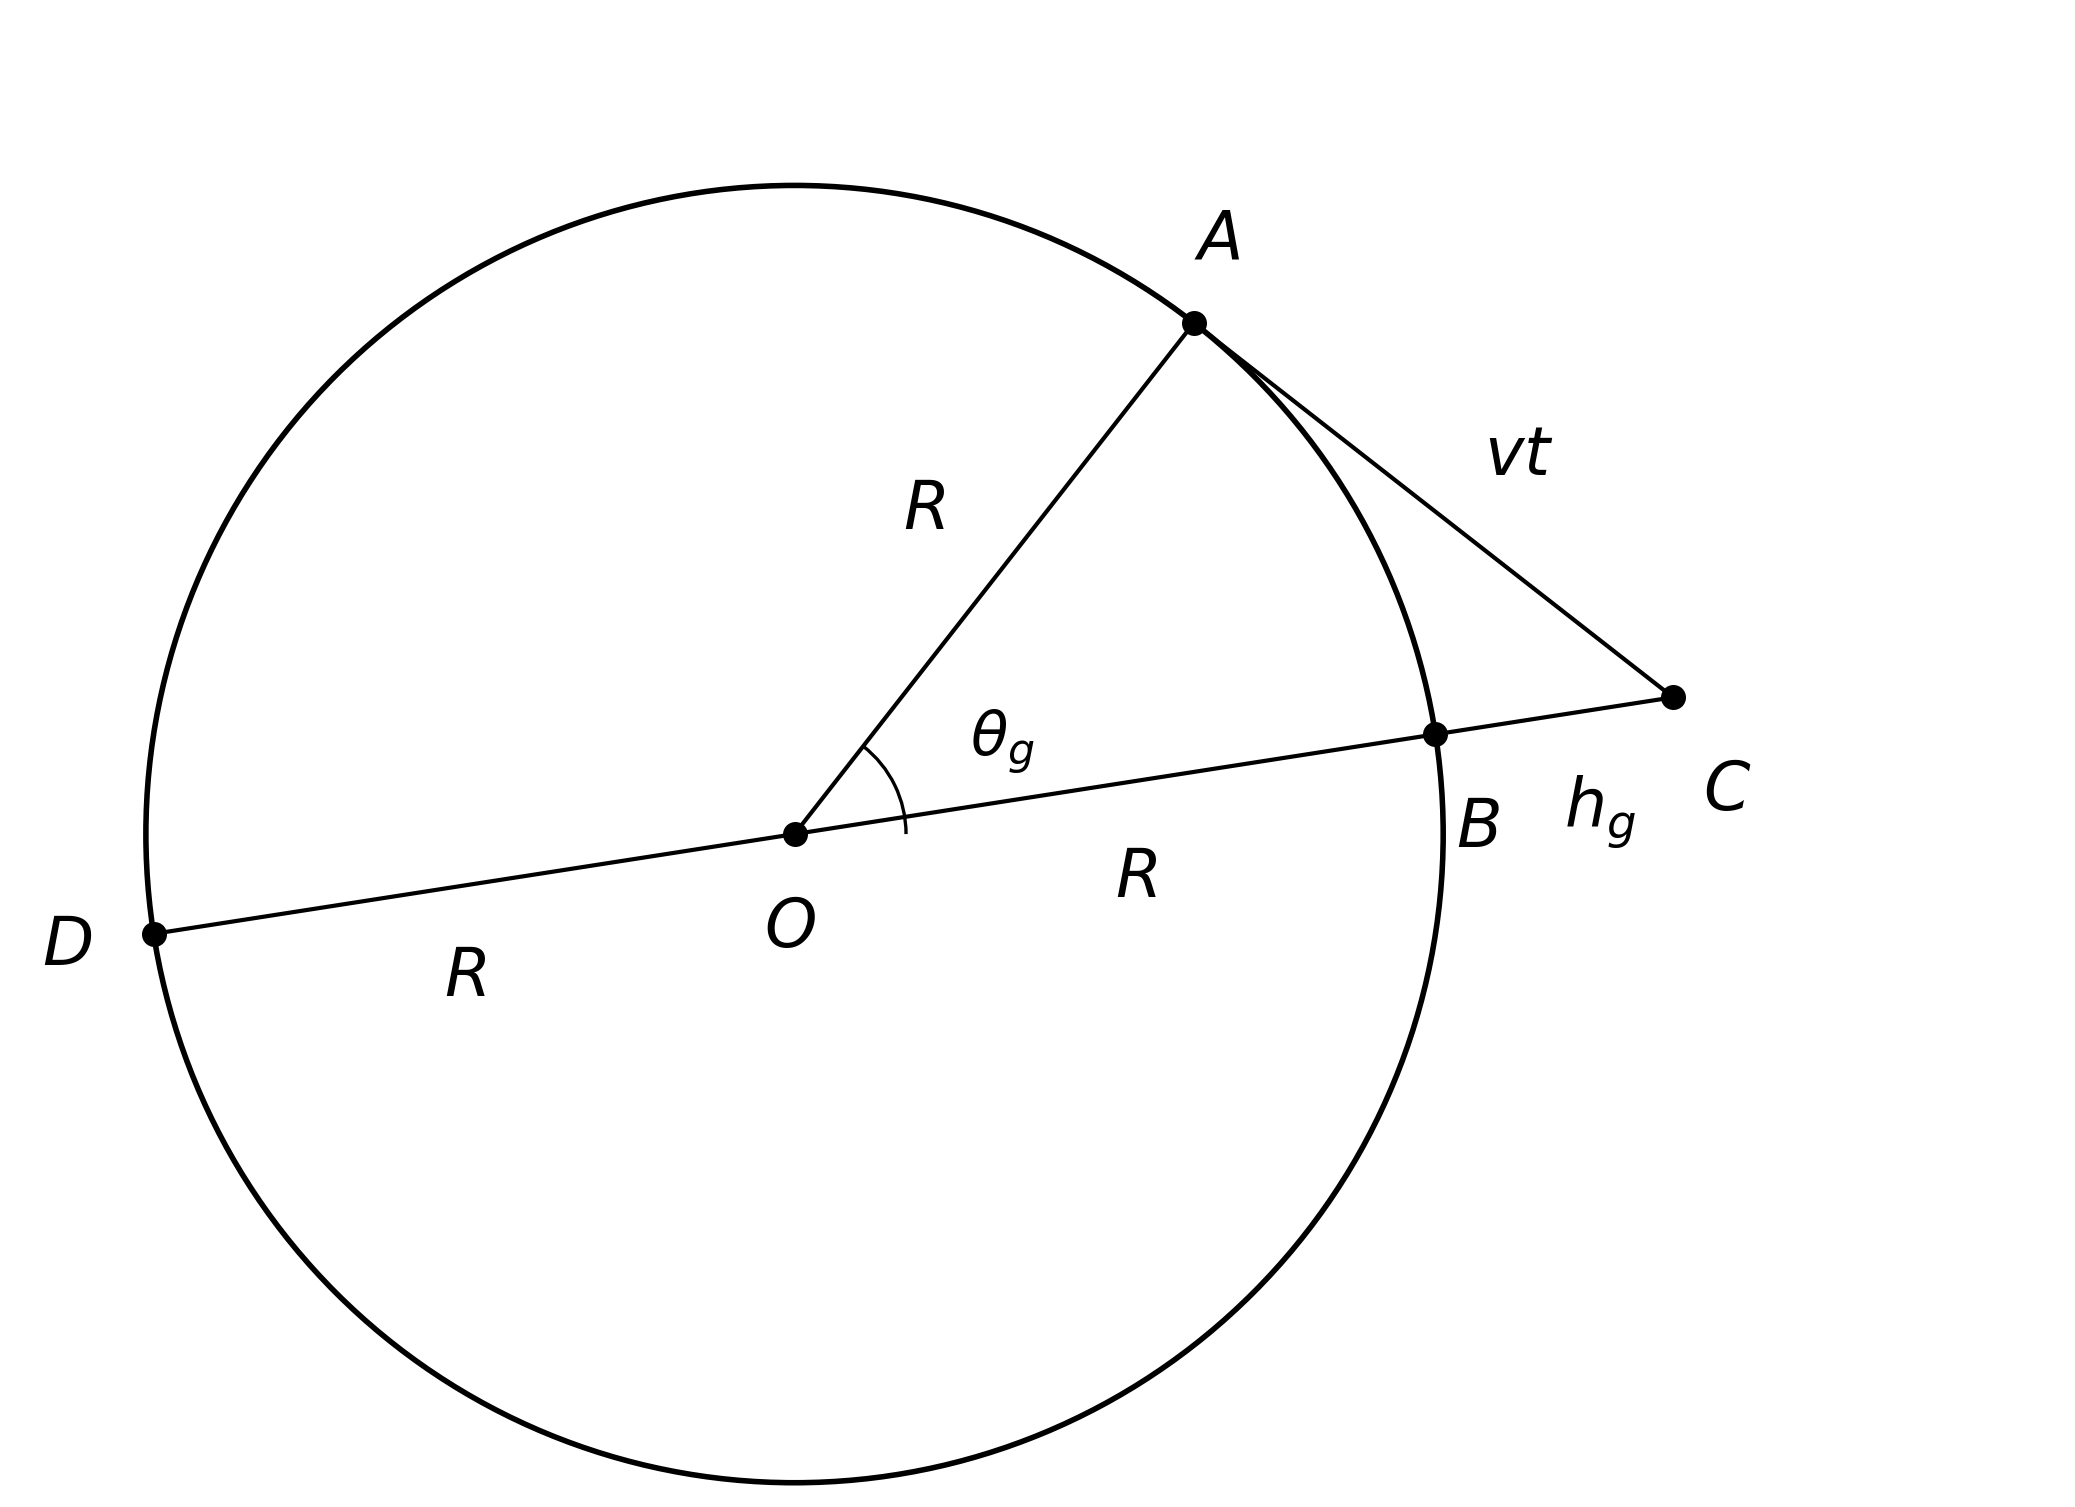
\includegraphics[width=0.7\textwidth]{centripetal_fig1.png}
\caption{Construção tangencial auxiliar que define o desvio geométrico $h_g$.}
\label{fig:centripetal}
\end{figure}

\begin{proposition}[Construção tangencial e potência do ponto exterior]
\label{prop:centripetal-power}
Seja uma circunferência de centro $\pt{O}$ e raio $R$. Em $\pt{A}$ sobre a circunferência, seja $\seg{AC}$ tangente, com $\seglen{AC}=vt$. Para toda secante que passa pelo ponto exterior $\pt{C}$ e intersecta a circunferência em $\pt{X}$ e $\pt{Y}$,
\be
\seglen{CX}\,\seglen{CY}=(vt)^2.
\label{eq:family-power}
\ee
Para a secante diametral que passa por $\pt{C},\pt{B},\pt{O},\pt{D}$ na Figura~\ref{fig:centripetal}, com $h_g=\seglen{CB}$, essa relação torna-se
\be
h_g(2R+h_g)=(vt)^2.
\label{eqtheo1}
\ee
\end{proposition}

\begin{proof}
Como $\seg{CA}$ é tangente à circunferência em $\pt{A}$, a Proposição \ref{popsectan} fornece, para qualquer secante que passa por $\pt{C}$ e intersecta a circunferência em $\pt{X}$ e $\pt{Y}$,
\be
\seglen{CX}\,\seglen{CY}=\seglen{CA}^{2}.
\ee
Usando a Equação~\eqref{eq:tangent-length}, o valor comum é $(vt)^2$, o que demonstra a Equação~\eqref{eq:family-power}. Escolhendo a secante que passa pelo centro, obtêm-se $\seglen{CB}=h_g$ e $\seglen{CD}=2R+h_g$, portanto
\be
h_g(2R+h_g)=(vt)^2.
\ee
Essa é a especialização diametral desejada da relação de potência invariante em relação à secante.
\end{proof}

A mesma identidade também pode ser verificada independentemente a partir do triângulo retângulo $\triangle \mathbf{OAC}$: como $\seg{OA}\perp\seg{AC}$,
\be
(R+h_g)^2=R^2+(vt)^2,
\label{pytha}
\ee
que se fatora na Equação~\eqref{eqtheo1}. O papel lógico do teorema da potência de um ponto é, contudo, mais amplo do que essa verificação: a Equação~\eqref{eq:family-power} afirma que o produto independe da secante escolhida através de $\pt{C}$, ao passo que o cálculo pitagórico trata apenas da secante diametral particular. Na notação do Apêndice~\ref{app:power-point}, o ponto exterior possui, portanto, a potência exata
\be
\Pot_{\lambda}(\pt{C})=\seglen{CO}^{2}-R^2=\seglen{CA}^{2}=(vt)^2,
\label{eq:power-C}
\ee
onde $\lambda$ denota a órbita circular.

\section{Cinemática Circular Local e Aceleração Centrípeta}\label{sec:local-kinematics}

A relação entre desvio normal e aceleração normal é formulada de modo mais claro como uma propriedade local da trajetória física. Escolha a origem do tempo de modo que a partícula esteja no ponto $\pt{A}$ quando $t=0$ e denote por $\mathbf{r}(t)$ seu vetor posição. Suponha que $\mathbf{r}$ seja de classe $C^3$ em uma vizinhança de $t=0$. A expansão de Taylor em torno de $t=0$ é então
\be
\mathbf{r}(t)=\mathbf{r}_{\pt{A}}
+\left.\frac{\dd\mathbf{r}}{\dd t}\right|_{t=0}t
+\frac{1}{2}\left.\frac{\dd^2\mathbf{r}}{\dd t^2}\right|_{t=0}t^2
+O(t^3).
\label{eq:trajectory-taylor}
\ee
A velocidade e a aceleração instantâneas em $\pt{A}$ são, portanto, definidas separadamente por
\begin{subequations}\label{eq:va-aa-definitions}
\begin{align}
\mathbf{v}_{\pt{A}}&\equiv\left.\frac{\dd\mathbf{r}}{\dd t}\right|_{t=0},
\label{eq:velocity-A}\\
\mathbf{a}_{\pt{A}}&\equiv\left.\frac{\dd^2\mathbf{r}}{\dd t^2}\right|_{t=0}.
\label{eq:acceleration-A}
\end{align}
\end{subequations}
Seja $\mathbf{t}_{\pt{A}}=\mathbf{v}_{\pt{A}}/v$ o vetor tangente unitário à órbita em $\pt{A}$ e seja $\mathbf{n}_{\pt{A}}$ o vetor normal unitário dirigido para o interior, isto é, para o centro $\pt{O}$. Esses vetores são ortogonais, $\mathbf{t}_{\pt{A}}\!\cdot\!\mathbf{n}_{\pt{A}}=0$, e formam o referencial tangente--normal local. A aceleração pode, consequentemente, ser decomposta como
\be
\mathbf{a}_{\pt{A}}=a_t\,\mathbf{t}_{\pt{A}}+a_n\,\mathbf{n}_{\pt{A}},
\label{eq:acc-decomposition}
\ee
onde $a_t=\mathbf{t}_{\pt{A}}\!\cdot\!\mathbf{a}_{\pt{A}}$ é a componente tangencial e a componente normal dirigida para o interior é
\be
 a_n\equiv\mathbf{n}_{\pt{A}}\!\cdot\!\mathbf{a}_{\pt{A}}.
\label{eq:normal-acc-component}
\ee
Os termos de ordem zero e de primeira ordem da Equação~\eqref{eq:trajectory-taylor} também possuem uma interpretação geométrica direta. Se a interação dirigida para o interior fosse removida em $\pt{A}$, a partícula conservaria sua velocidade instantânea e, após um intervalo $t$, alcançaria o ponto tangencial $\pt{C}$ da Figura~\ref{fig:centripetal}. A continuação tangencial inercial correspondente tem posição
\be
\mathbf{r}^{\mathrm{tan}}_{\pt{C}}(t)=\mathbf{r}_{\pt{A}}+\mathbf{v}_{\pt{A}}t.
\label{eq:tangent-continuation}
\ee
A partícula real, por sua vez, alcança um ponto $\pt{Q}$ sobre a órbita circular, com posição $\mathbf{r}(t)$. O vetor
\be
\Delta\mathbf{r}(t)\equiv\mathbf{r}(t)-\mathbf{r}^{\mathrm{tan}}_{\pt{C}}(t).
\label{eq:delta-r}
\ee
Portanto, ele mede o afastamento da trajetória física em relação à continuação tangencial inercial. No referencial tangente--normal local, $\Delta\mathbf{r}$ decompõe-se em projeções tangencial e normal mutuamente ortogonais. Geometricamente, essas projeções são os dois catetos de um triângulo retângulo cuja hipotenusa é $\Delta\mathbf{r}$. Como $\mathbf{n}_{\pt{A}}$ é um vetor unitário perpendicular a $\mathbf{t}_{\pt{A}}$, o produto escalar com $\mathbf{n}_{\pt{A}}$ elimina a projeção tangencial e fornece precisamente o cateto normal dirigido para o interior, com sinal. Definimos, portanto, o afastamento normal local por
\be
h_c(t)\equiv\mathbf{n}_{\pt{A}}\!\cdot\!\Delta\mathbf{r}(t)
=\mathbf{n}_{\pt{A}}\!\cdot\!\left[\mathbf{r}(t)-\mathbf{r}_{\pt{A}}-\mathbf{v}_{\pt{A}}t\right].
\label{eq:normal-departure-definition}
\ee
Substituindo a expansão de Taylor e utilizando a Equação~\eqref{eq:normal-acc-component}, obtém-se
\be
h_c(t)=\frac{1}{2}a_n t^2+O(t^3).
\label{eq:normal-departure}
\ee
No movimento circular uniforme, o módulo da velocidade é constante. Assim,
\be
\frac{\dd}{\dd t}\!\left(\mathbf{v}\!\cdot\!\mathbf{v}\right)
=2\,\mathbf{v}\!\cdot\!\mathbf{a}=0,
\label{eq:constant-speed-orthogonality}
\ee
de modo que a aceleração não possui componente tangencial. Como a trajetória circular se curva em direção ao centro, a componente normal restante aponta ao longo de $\mathbf{n}_{\pt{A}}$. Na terminologia newtoniana, essa componente instantânea dirigida para o interior é a aceleração centrípeta; a relação não trivial para seu módulo não é assumida aqui, mas será obtida a partir da construção geométrica. Definimos, portanto,
\be
 a_c\equiv a_n=\mathbf{n}_{\pt{A}}\!\cdot\!\mathbf{a}_{\pt{A}}>0.
\label{eq:centripetal-definition}
\ee
Com essa definição, a Equação~\eqref{eq:normal-departure} torna-se $h_c(t)=\tfrac12 a_c t^2+O(t^3)$ e, portanto,
\be
 a_c=\lim_{t\to0}\frac{2h_c(t)}{t^2}.
\label{eq:normal-acc-definition}
\ee
A Equação~\eqref{eq:normal-acc-definition} é uma afirmação instantânea: ela não supõe que a aceleração permaneça constante ao longo de um intervalo finito. Ainda assim, identifica a aceleração normal como duas vezes o coeficiente quadrático que governa a separação entre a trajetória física e sua tangente no limite de um intervalo de tempo arbitrariamente curto. Essa é a forma local moderna da ideia geométrica de limite subjacente aos tratamentos newtonianos do movimento centrípeto \cite{newton1729principia,erlichson1991motive}. O desvio geométrico auxiliar $h_g$, introduzido na Equação~\eqref{eq:hg-definition}, é distinto de $h_c$: $h_g$ é o intervalo radial entre a extremidade tangencial $\pt{C}$ e a circunferência, medido ao longo da semirreta que passa por $\pt{C}$ e $\pt{O}$, ao passo que $h_c$ é o afastamento normal, dirigido para o interior, do ponto orbital real $\pt{Q}$ em relação à continuação tangencial em $\pt{A}$. As duas grandezas não são medidas na mesma direção nem têm como referência o mesmo ponto; sua relação deve, portanto, ser estabelecida, e não suposta.

O movimento uniforme fornece a cinemática restante. A distância percorrida ao longo da circunferência no tempo $t$ é $s=vt$, enquanto $s=R\theta$. Introduza o parâmetro adimensional de tempo curto
\be
\tau\equiv\frac{vt}{R},
\label{eq:tau}
\ee
de modo que a posição angular física após o tempo $t$ seja $\theta=\tau$. Em contraste, o ponto auxiliar $\pt{B}$ pertence à semirreta que passa por $\pt{O}$ e $\pt{C}$, e o ângulo correspondente na Figura~\ref{fig:centripetal} é $\theta_g$. A partir do triângulo retângulo $\triangle \mathbf{OAC}$,
\be
\theta_g=\arctan\tau.
\label{eq:theta-g}
\ee
Para qualquer intervalo de tempo finito, portanto, o ângulo auxiliar é $\theta_g=\arctan\tau$, enquanto o ângulo orbital físico é $\theta=\tau$; em geral, os dois não são iguais. Substituir $\arctan\tau$ por $\tau$ constitui uma aproximação de pequenos ângulos, justificada apenas no regime local $|\tau|=|vt|/R\ll1$, e não pode ser aplicada a um valor finito arbitrário de $t$. Consequentemente, o ponto auxiliar $\pt{B}$ não pode, em geral, ser identificado com o ponto orbital físico $\pt{Q}$. No limite local,
\be
\arctan\tau=\tau-\frac{\tau^3}{3}+O(\tau^5),
\ee
de modo que a distinção angular desaparece em primeira ordem. O coeficiente quadrático crucial, entretanto, já pode ser obtido diretamente da relação exata de potência antes de qualquer expansão em série. Dividindo a Equação~\eqref{eqtheo1} por $t^2$, obtém-se
\be
\left(2R+h_g\right)\frac{h_g}{t^2}=v^2.
\ee
Como $h_g\to0$ quando $t\to0$,
\be
\lim_{t\to0}\frac{2h_g}{t^2}=\frac{v^2}{R}.
\label{eq:hg-limit}
\ee
Assim, a construção baseada na potência de um ponto determina o coeficiente quadrático do desvio auxiliar independentemente de qualquer identificação, em tempo finito, de $\pt{B}$ com a órbita física.

Os desvios geométrico e físico podem agora ser comparados explicitamente. O desvio geométrico decorre exatamente da Equação~\eqref{eqtheo1}, ou, de forma equivalente, da Equação~\eqref{pytha}:
\be
h_g=\sqrt{R^2+v^2t^2}-R=R\left(\sqrt{1+\tau^2}-1\right),
\label{eq:hg-exact}
\ee
com expansão para tempos curtos
\be
h_g=\frac{v^2t^2}{2R}-\frac{v^4t^4}{8R^3}+O(t^6).
\label{eq:hg-expansion}
\ee
Para escrever explicitamente o desvio normal físico, escolha coordenadas cartesianas com $\pt{O}=(0,0)$, $\pt{A}=(R,0)$ e reta tangente $x=R$. O ponto orbital real após o deslocamento angular $\theta=\tau$ é
\be
\pt{Q}=(R\cos\tau,R\sin\tau),
\label{eq:Q-coordinate}
\ee
e sua distância à reta tangente, medida ao longo da normal dirigida para o interior, é
\be
h_c=R-R\cos\tau=R(1-\cos\tau),
\label{eq:hc-exact}
\ee
o que fornece
\be
h_c=\frac{v^2t^2}{2R}-\frac{v^4t^4}{24R^3}+O(t^6).
\label{eq:hc-expansion}
\ee
Consequentemente,
\be
h_g-h_c=-\frac{v^4t^4}{12R^3}+O(t^6).
\label{eq:deviation-error}
\ee
Os dois desvios não são iguais em tempo finito, mas sua diferença é de quarta ordem e, portanto,
\be
\lim_{t\to0}\frac{2(h_g-h_c)}{t^2}=0.
\ee
Combinando esse resultado com a Equação~\eqref{eq:hg-limit}, obtém-se
\be
\lim_{t\to0}\frac{2h_c}{t^2}=\lim_{t\to0}\frac{2h_g}{t^2}=\frac{v^2}{R}.
\label{eq:local-equivalence}
\ee
Usando a Equação~\eqref{eq:normal-acc-definition}, obtém-se
\be
a_c=\frac{v^2}{R},
\ee
com direção para o centro da circunferência. Nessa ordem de argumentos, a identidade tangente--secante fornece o coeficiente quadrático do desvio auxiliar, e a Equação~\eqref{eq:deviation-error} justifica a transferência desse coeficiente para a trajetória circular física. Uma medida adimensional da discrepância em tempo finito é obtida normalizando-se pelo desvio físico:
\be
\varepsilon(\tau)\equiv\frac{h_g-h_c}{h_c}=\frac{\sqrt{1+\tau^2}+\cos\tau-2}{1-\cos\tau}=-\frac{\tau^2}{6}+O(\tau^4).
\label{eq:relative-error}
\ee
Essa expressão torna quantitativa a qualificação de tempo curto sem alterar o papel da construção. Para ilustrar, se for adotada uma tolerância de $1\%$, $|\varepsilon(\tau)|=0.01$, a expressão exata da Equação~\eqref{eq:relative-error} fornece $\tau\simeq0.249876$, correspondente a um ângulo orbital de aproximadamente $14.32^{\circ}$. O limiar numérico não é intrínseco à derivação; ele apenas fornece uma escala para a afirmação assintótica. Essa distinção preserva o conteúdo pedagógico da construção clássica, ao mesmo tempo que separa duas afirmações logicamente distintas. A igualdade $\seglen{CA}^{2}=\seglen{CX}\,\seglen{CY}$ é um invariante exato da geometria euclidiana da circunferência. Seu uso na cinemática circular é local porque a interseção auxiliar selecionada por uma secante particular não precisa coincidir com o ponto orbital em tempo finito. O que permanece no limite de tempos curtos é o afastamento comum de segunda ordem em relação à tangente, e esse coeficiente é precisamente a aceleração centrípeta.

\begin{remark}[Potência associada à extremidade tangencial]
\label{rem:ac-power}
A Equação~\eqref{eq:power-C} mostra que o quadrado do deslocamento tangencial $\seglen{AC}^{2}=(vt)^2$ é a potência do ponto exterior $\pt{C}$ em relação à órbita circular. A Equação~\eqref{eq:family-power} acrescenta a afirmação geometricamente mais forte de que o mesmo valor é obtido para toda secante que passa por $\pt{C}$. A secante diametral não é, portanto, a definição da correspondência, mas o membro mais conveniente de uma família de secantes para expressar o produto em termos de $R$ e $h_g$.
\end{remark}

\section{Conclusão}

Este trabalho examinou uma via geométrica clássica para a aceleração centrípeta e sua correspondência com a relação tangente--secante na geometria da circunferência. A atribuição histórica exige uma distinção clara: as relações subjacentes entre produtos de segmentos são euclidianas, enquanto a contribuição de Steiner em 1826 \cite{steiner1826einige} introduziu a potência de um ponto como grandeza unificadora. O tratamento newtoniano do movimento circular pertence, portanto, a uma tradição geométrica muito anterior à terminologia do século XIX, embora a linguagem moderna da potência de um ponto forneça uma maneira eficiente de descrever a estrutura da construção. Para a extremidade tangencial $\pt{C}$, a afirmação geométrica exata é que $\Pot_{\lambda}(\pt{C})=\seglen{CA}^{2}=\seglen{CX}\,\seglen{CY}=(vt)^2$ para toda secante que passa por $\pt{C}$ e intersecta a circunferência em $\pt{X}$ e $\pt{Y}$. A secante diametral é o membro conveniente dessa família para o qual o produto se torna $h_g(2R+h_g)$. Assim, a fatoração pitagórica do triângulo retângulo $\triangle \mathbf{OAC}$ verifica a configuração selecionada. Ao mesmo tempo, a formulação pela potência de um ponto identifica o invariante comum compartilhado por toda a família de secantes. A interpretação física é local, e não exata em tempo finito. O ponto auxiliar $\pt{B}$ e o ponto orbital físico $\pt{Q}$ possuem posições angulares $\theta_g=\arctan\tau$ e $\theta=\tau$, respectivamente, com $\tau=vt/R$. Correspondentemente, $h_g$ é um intervalo radial medido ao longo da semirreta que passa por $\pt{O}$ e $\pt{C}$, enquanto $h_c$ é a distância normal de $\pt{Q}$ à tangente em $\pt{A}$. Sua diferença começa na quarta ordem, $h_g-h_c=-v^4t^4/(12R^3)+O(t^6)$, e sua discrepância relativa satisfaz $\varepsilon(\tau)=-\tau^2/6+O(\tau^4)$. Uma tolerância de $1\%$ em $|\varepsilon|$ corresponde a $\tau\simeq0.249876$, ou a um ângulo orbital de aproximadamente $14.32^{\circ}$. Ainda assim, a relação exata de potência fixa o coeficiente quadrático comum, e a expansão local da trajetória fornece então a conhecida aceleração centrípeta $a_c=v^2/R$. A distinção entre identidade euclidiana exata e interpretação física local constitui, portanto, a qualificação central estabelecida pela construção.

O valor pedagógico do argumento reside em demonstrar a relação entre movimento inercial, curvatura e geometria clássica da circunferência antes da introdução de ferramentas analíticas mais avançadas. A literatura histórica e pedagógica revisada na Seção 2 mostra que esse objetivo motivou derivações baseadas no deslocamento em relação à tangente, em trigonometria, no espaço das velocidades e em reconstruções históricas. O presente tratamento conserva as demonstrações clássicas no Apêndice~\ref{app:power-point}, ao mesmo tempo que explicita os papéis distintos da geometria euclidiana, da linguagem invariante posterior de Steiner e da cinemática circular local. Não se reivindica aqui qualquer validação em sala de aula ou estudo educacional comparativo.

\bibliographystyle{unsrturl}
\bibliography{centripetal}



% Continuidade editorial: referencias e apendice sem quebra de pagina forcada.
\appendix
\setcounter{subsection}{0}
\renewcommand{\thesubsection}{A.\arabic{subsection}}
\setcounter{figure}{0}
\renewcommand{\thefigure}{A.\arabic{figure}}
\renewcommand{\theproposition}{A.\arabic{proposition}}
\section{Potência de um Ponto na Geometria Clássica da Circunferência}\label{app:power-point}

\subsection{Esclarecimento histórico e notação}

As relações entre produtos de segmentos utilizadas neste artigo pertencem à geometria euclidiana clássica da circunferência. Em particular, as configurações de cordas que se intersectam e de tangente--secante aparecem nos \textit{Elementos} de Euclides, Livro III, Proposições 35 e 36 \cite{euclid1956elements}. A contribuição de Steiner em 1826 \cite{steiner1826einige} foi de outra natureza: ele introduziu a noção de potência como uma grandeza associada a um ponto e a uma circunferência, fornecendo assim uma interpretação algébrica unificada dessas configurações clássicas. A mecânica geométrica de Newton, portanto, antecede Steiner e foi desenvolvida em uma tradição matemática na qual os resultados euclidianos subjacentes já estavam disponíveis. Para completar a exposição e manter autocontida a correspondência subsequente, recordamos brevemente as demonstrações clássicas das relações entre produtos de segmentos empregadas na Seção~\ref{sec:exact-geometry}. Esses resultados são padrão; sua inclusão neste apêndice tem por objetivo fixar a notação e explicitar a estrutura geométrica requerida pelo argumento físico. Ao longo desta seção, os rótulos dos pontos são apresentados em negrito romano, e $\seglen{XY}$ denota o comprimento positivo usual do segmento que une $\pt{X}$ e $\pt{Y}$. Quando segmentos orientados forem introduzidos adiante, $\dseg{XY}$ denotará o segmento correspondente com sinal ao longo de uma secante orientada. As três configurações euclidianas consideradas abaixo não são resultados independentes, mas diferentes manifestações da mesma estrutura de produtos de segmentos. Primeiro as recordamos em sua forma usual com comprimentos positivos e, em seguida, as reunimos na formulação com sinal da potência de um ponto.

\subsection{Configurações clássicas de produtos de segmentos}

A Figura~\ref{steinerpop} resume as três configurações geométricas usuais. A primeira envolve duas cordas que se intersectam no interior da circunferência; a segunda envolve duas secantes traçadas a partir de um ponto exterior; a terceira é o caso limite tangente--secante. As demonstrações são incluídas apenas para tornar explícita e autocontida a correspondência mecânica utilizada posteriormente.

\begin{figure}[H]
    \centering
    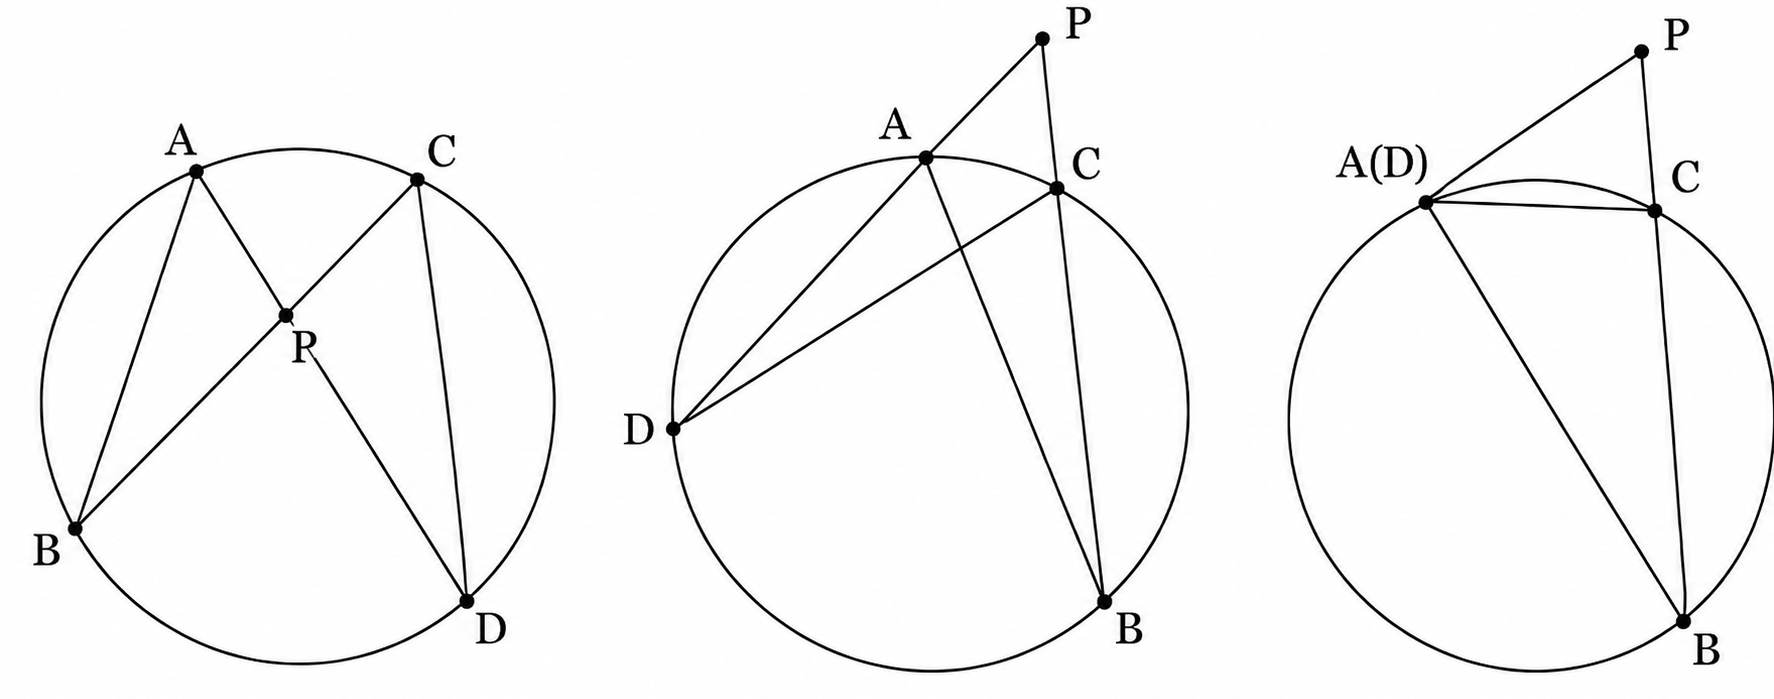
\includegraphics[width=0.82\textwidth]{steinerpop.png}
    \caption{Configurações clássicas de cordas que se intersectam, secantes a partir de um ponto exterior e tangente--secante.}
    \label{steinerpop}
\end{figure}

\begin{proposition}[Cordas que se intersectam]
\label{pop2chords}
Sejam $\seg{AD}$ e $\seg{CB}$ duas cordas de uma circunferência que se intersectam em um ponto interior $\pt{P}$, como mostrado no primeiro painel da Figura~\ref{steinerpop}. Então
\be
\seglen{AP}\,\seglen{DP}=\seglen{BP}\,\seglen{CP}.
\ee
\end{proposition}

\begin{proof}
Considere $\triangle \mathbf{ABP}$ e $\triangle \mathbf{CDP}$. Os ângulos $\angle \mathbf{ABP}$ e $\angle \mathbf{CDP}$ subtendem a mesma corda $\seg{AC}$, enquanto $\angle \mathbf{APB}$ e $\angle \mathbf{CPD}$ são opostos pelo vértice. Logo, $\triangle \mathbf{ABP}\sim\triangle \mathbf{CDP}$, de modo que
\be
\frac{\seglen{AP}}{\seglen{CP}}=\frac{\seglen{BP}}{\seglen{DP}},
\ee
o que fornece $\seglen{AP}\,\seglen{DP}=\seglen{BP}\,\seglen{CP}$.
\end{proof}

A identidade para cordas que se intersectam já exibe a estrutura invariante essencial. Uma vez fixado o ponto de interseção, o produto das duas distâncias orientadas ao longo de uma reta é igual ao produto correspondente ao longo da outra. Para um ponto interior, entretanto, o uso de comprimentos positivos usuais oculta o sinal que posteriormente aparece de modo natural na definição de potência.

\begin{proposition}[Duas secantes a partir de um ponto exterior]
\label{pop2sec}
Seja $\pt{P}$ um ponto exterior a uma circunferência. Sejam duas secantes traçadas a partir de $\pt{P}$ que intersectam a circunferência em $\pt{A},\pt{D}$ e $\pt{C},\pt{B}$, respectivamente, com $\pt{A}$ e $\pt{C}$ sendo os pontos de interseção mais próximos de $\pt{P}$, como mostrado no segundo painel da Figura~\ref{steinerpop}. Então
\be
\seglen{PA}\,\seglen{PD}=\seglen{PC}\,\seglen{PB}.
\ee
\end{proposition}

\begin{proof}
Considere $\triangle \mathbf{PAB}$ e $\triangle \mathbf{PCD}$. Eles compartilham o ângulo em $\pt{P}$, e os demais ângulos relevantes são iguais porque os ângulos inscritos correspondentes subtendem a mesma corda $\seg{DB}$. Portanto, $\triangle \mathbf{PAB}\sim\triangle \mathbf{PCD}$, o que fornece
\be
\frac{\seglen{PA}}{\seglen{PC}}=\frac{\seglen{PB}}{\seglen{PD}},
\ee
e, portanto, $\seglen{PA}\,\seglen{PD}=\seglen{PC}\,\seglen{PB}$.
\end{proof}

Para um ponto exterior, ambos os fatores em cada produto são positivos quando se utilizam comprimentos usuais. Essa é a forma mais diretamente relacionada à construção empregada na Seção~\ref{sec:exact-geometry}.

\begin{proposition}[Forma tangente--secante]
\label{popsectan}
Seja $\pt{P}$ um ponto exterior a uma circunferência. Seja $\seg{PA}$ tangente à circunferência em $\pt{A}$, e seja uma secante traçada a partir de $\pt{P}$ que intersecta a circunferência primeiro em $\pt{C}$ e depois em $\pt{B}$, como mostrado no terceiro painel da Figura~\ref{steinerpop}. Então
\be
\seglen{PC}\,\seglen{PB}=\seglen{PA}^{2}.
\ee
\end{proposition}

\begin{proof}
Considere $\triangle \mathbf{PAC}$ e $\triangle \mathbf{PBA}$. O ângulo em $\pt{P}$ é comum. Pelo teorema do ângulo entre tangente e corda, o ângulo entre a tangente $\seg{PA}$ e a corda $\seg{AC}$ é igual ao ângulo inscrito que subtende a mesma corda; portanto, os triângulos são semelhantes. Assim,
\be
\frac{\seglen{PA}}{\seglen{PB}}=\frac{\seglen{PC}}{\seglen{PA}},
\ee
o que fornece $\seglen{PA}^{2}=\seglen{PC}\,\seglen{PB}$.
\end{proof}

A forma tangente--secante é a configuração requerida posteriormente. Sua relevância não reside apenas no fato de uma secante particular reproduzir o quadrado do comprimento da tangente, mas em que toda secante que passa pelo mesmo ponto exterior fornece o mesmo produto de segmentos. Essa invariância em relação à secante é o conteúdo geométrico que se torna especialmente transparente na linguagem da potência de um ponto.

\subsection{Potência de um ponto com sinal}

As três configurações acima podem ser unificadas introduzindo-se a potência de um ponto com sinal. Seja $\lambda$ uma circunferência de centro $\pt{O}$ e raio $R$. A potência de um ponto $\pt{P}$ em relação a $\lambda$ é
\be
\Pot_{\lambda}(\pt{P})=\seglen{PO}^{2}-R^2.
\label{eq:power-definition}
\ee
Portanto,
\be
\begin{cases}
\Pot_{\lambda}(\pt{P})>0, & \text{se } \pt{P} \text{ está fora da circunferência }(\seglen{PO}>R),\\[4pt]
\Pot_{\lambda}(\pt{P})=0, & \text{se } \pt{P} \text{ está sobre a circunferência }(\seglen{PO}=R),\\[4pt]
\Pot_{\lambda}(\pt{P})<0, & \text{se } \pt{P} \text{ está no interior da circunferência }(\seglen{PO}<R).
\end{cases}
\ee
Para um ponto exterior, os comprimentos positivos usuais fornecem
\be
\Pot_{\lambda}(\pt{P})=\seglen{PA}\,\seglen{PD}=\seglen{PC}\,\seglen{PB},
\ee
e, para uma tangente,
\be
\Pot_{\lambda}(\pt{P})=\seglen{PT}^{2}.
\ee
Para um ponto interior, a relação entre cordas escrita com comprimentos positivos permanece positiva, enquanto a potência com sinal é negativa:
\be
\Pot_{\lambda}(\pt{P})=-\seglen{PA}\,\seglen{PD}=-\seglen{PB}\,\seglen{PC}.
\ee
A diferença de sinal é puramente geométrica: para um ponto interior, as duas interseções de qualquer secante situam-se em lados opostos de $\pt{P}$. Segmentos orientados fornecem, portanto, uma maneira natural de absorver o sinal no próprio produto. Oriente cada reta secante e interprete $\dseg{PX}$ como a diferença de coordenadas com sinal de $\pt{P}$ até $\pt{X}$ ao longo dessa reta orientada. A relação pode então ser escrita uniformemente como
\be
\dseg{PA}\,\dseg{PD}=\dseg{PB}\,\dseg{PC}=\Pot_{\lambda}(\pt{P}).
\label{eq:directed-power}
\ee
A Figura~\ref{steinerpop2} ilustra três interpretações complementares utilizando comprimentos positivos usuais. No painel (a), $\pt{P}$ está fora da circunferência e $\seg{PT}$ é tangente em $\pt{T}$, de modo que a potência é positiva e igual a $\seglen{PT}^{2}$. No painel (b), $\pt{P}$ está no interior da circunferência e $\seg{PS}$ é perpendicular a $\seg{PO}$, com $\pt{S}$ sobre a circunferência; o triângulo retângulo $\triangle \mathbf{OPS}$ fornece $\seglen{PS}^{2}=R^2-\seglen{PO}^{2}=-\Pot_{\lambda}(\pt{P})$. No painel (c), $\pt{P}$ está fora da circunferência e uma secante a intersecta em $\pt{S}_1$ e $\pt{S}_2$, fornecendo $\seglen{PS_1}\,\seglen{PS_2}=\Pot_{\lambda}(\pt{P})$.

\begin{figure}[ht]
\centering
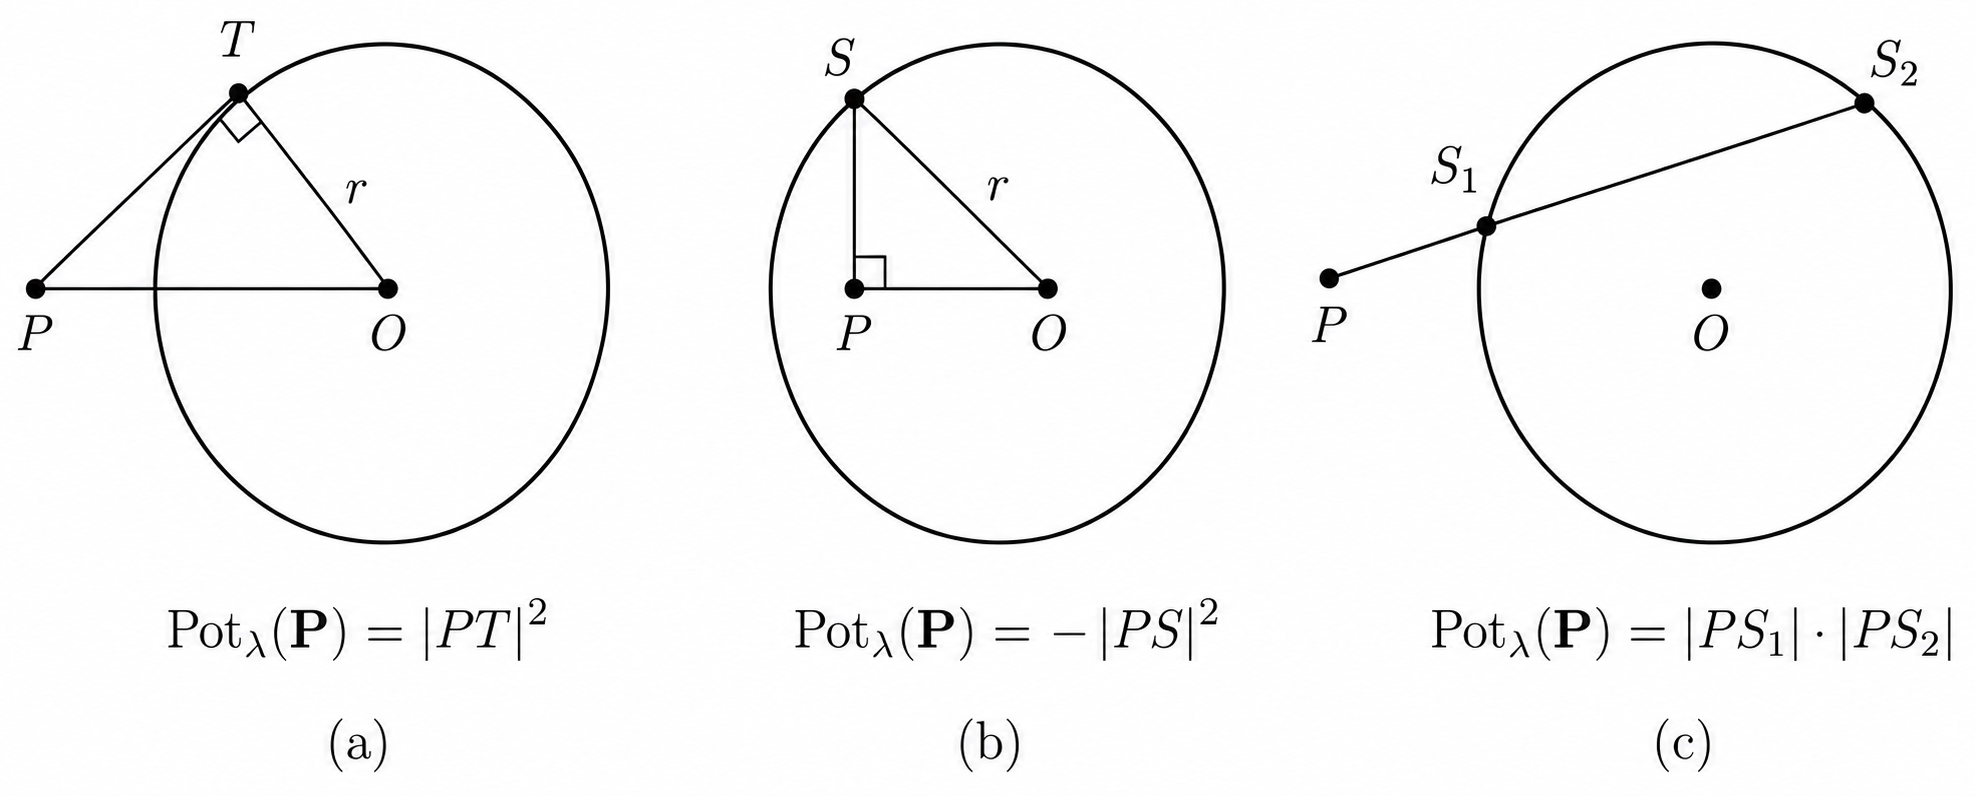
\includegraphics[scale=0.2]{steinerpop2.png}
\caption{Potência de um ponto com sinal em relação a uma circunferência de centro $\pt{O}$ e raio $R$. (a) Para um ponto exterior, $\Pot_{\lambda}(\pt{P})=\seglen{PT}^{2}>0$. (b) Para um ponto interior, $\Pot_{\lambda}(\pt{P})<0$ e $\seglen{PS}^{2}=-\Pot_{\lambda}(\pt{P})$. (c) Para uma secante exterior, $\Pot_{\lambda}(\pt{P})=\seglen{PS_1}\,\seglen{PS_2}>0$.}
\label{steinerpop2}
\end{figure}

O ponto central para a aplicação mecânica está agora explícito. O comprimento da tangente e todo produto de segmentos de secante que passa por um ponto exterior fixo representam a mesma grandeza invariante. A Seção~\ref{sec:exact-geometry} aplica precisamente essa forma para ponto exterior à extremidade tangencial gerada pelo movimento inercial.

\end{document}
